\documentclass[11pt]{article}

% Packages
\usepackage[utf8]{inputenc}
\usepackage[T1]{fontenc}
\usepackage{amsmath}
\usepackage{amsthm}
\usepackage{amssymb}
\usepackage{graphicx}
\usepackage{caption}
\usepackage{hyperref}
\hypersetup{colorlinks=true, linkcolor=blue, citecolor=blue, urlcolor=blue}
\usepackage{url}
\usepackage[numbers]{natbib}
\usepackage{geometry}
\geometry{margin=1in}

% Custom commands
\renewcommand{\v}[1]{\boldsymbol{#1}}

% Theorem environments
\newtheorem{theorem}{Theorem}[section]
\newtheorem{property}{Property}[section]
\newtheorem{remark}{Remark}[section]

% Title and author information
\title{When Does Model Simplification Matter?\\Consequence Analysis for Weibull Series Systems}
\author{
  \Large{Alex Towell} \\
  Department of Computer Science \\
  Southern Illinois University Edwardsville \\
  \href{mailto:lex@metafunctor.com}{lex@metafunctor.com} \\[4pt]
  ORCID: \href{https://orcid.org/0000-0001-6443-9897}{0000-0001-6443-9897}
}
\date{}

\begin{document}

\maketitle

\begin{abstract}
When a reliability engineer simplifies a series system model by assuming all components share a common Weibull shape parameter, how much accuracy is lost---and can the data even tell the difference? We show that these two questions have a quantitatively aligned answer. The common-shape model's prediction bias grows super-linearly with shape heterogeneity, remaining below 1\% in system MTTF through shape CV $\approx 15\%$, while the likelihood ratio test's power to detect the misspecification grows super-linearly. This creates a safe zone: the test lacks power precisely where the consequence of using the wrong model is negligible for engineering decisions. An adaptive LRT-based procedure exploits this alignment, achieving RMSE within 2.5\% of the full model at $n \geq 500$ while selecting the simpler model over 90\% of the time when appropriate. The common-shape model is the unique single-parameter reduction that preserves the Weibull property of the system lifetime, making it the natural parsimony boundary. Our analysis, conducted under realistic conditions of right-censored and masked failure data, provides practitioners with both the assurance that simplification is safe and the tools to decide when it is not.
\end{abstract}

\noindent\textbf{Keywords:} Weibull distribution, series systems, masked failure data, model selection, likelihood ratio test

\section{Introduction}

Consider a turbine engine whose operation depends on bearings, seals, and blades arranged in series---any component failure grounds the engine. Field maintenance logs record the failure time and a short list of suspect components (the candidate set), but exact root-cause analysis requires costly teardown. Warranty programs further right-censor units still in service. The engineer faces a fundamental modeling choice: a full model with separate Weibull shape and scale parameters for each of $m$ components ($2m$ parameters), or a reduced model that assumes a common shape parameter across all components ($m+1$ parameters).

The full model is more flexible but harder to estimate with limited masked data. The reduced model is more parsimonious and---uniquely among single-parameter reductions---renders the system lifetime itself Weibull \cite{barlow1975}, enabling closed-form reliability metrics. But is the simplification safe? The existing literature on this question focuses almost entirely on whether a likelihood ratio test can \emph{detect} the difference between models \cite{towell2023reliability}. This is the wrong question. The right question is: when the reduced model is wrong, does it produce predictions that are wrong enough to change an engineering decision?

This paper answers both questions and quantifies the alignment between them. The prediction bias of the common-shape model grows super-linearly with shape heterogeneity, while the LRT's power to detect that heterogeneity grows super-linearly. The consequence is negligible precisely where the test lacks power, and the test has high power precisely where the consequence warrants switching models. An adaptive procedure exploits this alignment to automatically select the appropriate model from data.

\subsection{Related Work}

The statistical treatment of masked system failure data originates with Usher and Hodgson \cite{Usher-1988}, who introduced maximum likelihood methods for component reliability estimation from masked system life-test data. Lin, Usher, and Guess \cite{Lin-1993} derived exact maximum likelihood estimators, while Lin, Usher, and Guess \cite{Lin-1996} developed Bayesian approaches. For Weibull components specifically, Usher \cite{Usher-1996} addressed reliability prediction with masked data, and Guess and Usher \cite{Joh-1989} proposed an iterative estimation approach. Sarhan \cite{Amma-2001, Amma-2004} extended the framework to various distributional assumptions, Tan \cite{Zhibi-2005} treated masked binomial system testing data, while Tan \cite{Zhibi-2007} contributed methods for exponential component reliability estimation. Guo, Niu, and Szidarovszky \cite{Huairu-2013} studied component reliability estimation from incomplete system failure data, providing the baseline system configuration used in our simulations. Towell \cite{towell2023reliability} developed a comprehensive likelihood model incorporating both right-censoring and candidate sets for Weibull series systems.

The closure property of the Weibull minimum under common shape is a classical result in reliability theory \cite{barlow1975, lawless2003, meeker1998}. Craiu and Lee \cite{Craiu-2005} addressed model selection for competing-risks models with and without masking, though not in the Weibull series system context. The model selection question---common shape versus heterogeneous shapes---has not, to our knowledge, been studied systematically for masked data, nor has the consequence of misspecification been quantified.

For general model selection methodology, we employ the likelihood ratio test \cite{wilks1938} and compare with the Akaike Information Criterion \cite{akaike1974} and Bayesian Information Criterion \cite{schwarz1978}. For a comprehensive treatment of information-theoretic model selection, see \cite{burnham2002}.

\subsection{Contributions}

\begin{enumerate}
\item \textbf{Bias-detectability alignment}: We quantify the alignment between the common-shape model's prediction bias and the LRT's detection power as functions of shape heterogeneity. MTTF bias remains below 1\% through CV $\approx 15\%$ (super-linear growth), while the LRT achieves 80\% power only at higher CVs (super-linear growth). The practical consequence: the wrong model choice is harmless exactly where it is likely.

\item \textbf{Consequence analysis}: We quantify the bias in system MTTF and reliability function predictions when the common-shape model is applied to systems with heterogeneous shapes. The 1\% MTTF bias threshold is not crossed until CV $\approx 20\%$. Surprisingly, a bias-variance decomposition reveals that the full model has lower MTTF variance than the reduced model even when the reduced model is correctly specified, because the nonlinear MTTF functional amplifies the constrained estimator's variance more than the unconstrained estimator's.

\item \textbf{Adaptive model selection}: We evaluate an LRT-based procedure that exploits the alignment, achieving RMSE within 2.5\% of the always-full strategy at $n \geq 500$ while selecting the simpler model $> 90\%$ of the time when the data support it.
\end{enumerate}

The paper is organized as follows. Section~\ref{sec:framework} presents the model framework. Section~\ref{sec:consequences} quantifies the consequences of model misspecification. Section~\ref{sec:lrt} characterizes the LRT. Section~\ref{sec:adaptive} develops the adaptive procedure. Section~\ref{sec:conclusion} concludes.

%% =========================================================================
\section{Model Framework}
\label{sec:framework}

\subsection{Series System with Weibull Components}

Consider a series system of $m$ independent components, where the system fails when any component fails. Each component lifetime $T_j$ follows a two-parameter Weibull distribution with shape $k_j > 0$ and scale $\lambda_j > 0$:
\begin{equation}
f_j(t; k_j, \lambda_j) = \frac{k_j}{\lambda_j}\left(\frac{t}{\lambda_j}\right)^{k_j-1} \exp\left\{-\left(\frac{t}{\lambda_j}\right)^{k_j}\right\}, \quad t > 0.
\end{equation}
The system lifetime $T = \min\{T_1, \ldots, T_m\}$ has reliability function, hazard function, and density:
\begin{align}
\label{eq:sys_reliability}
R(t;\v\theta) &= \exp\biggl\{-\sum_{j=1}^{m}\biggl(\frac{t}{\lambda_j}\biggr)^{k_j}\biggr\}, \\
\label{eq:sys_hazard}
h(t;\v\theta) &= \sum_{j=1}^{m} \frac{k_j}{\lambda_j}\biggl(\frac{t}{\lambda_j}\biggr)^{k_j-1}, \\
f(t;\v\theta) &= h(t;\v\theta) \cdot R(t;\v\theta),
\end{align}
where $\v\theta = (k_1, \lambda_1, \ldots, k_m, \lambda_m)$ is the full parameter vector.

The shape parameter governs the failure mode: $k_j < 1$ indicates decreasing hazard (infant mortality), $k_j = 1$ gives the exponential (constant hazard), and $k_j > 1$ gives increasing hazard (wear-out). The mean time to failure is $\text{MTTF}_j = \lambda_j \Gamma(1 + 1/k_j)$.

\subsection{Masked and Censored Data}

We observe $n$ independent system lifetimes under two forms of incomplete information:
\begin{itemize}
\item \textbf{Right-censoring}: Some systems are still operating at the end of the observation period. For system $i$, $\delta_i = 1$ indicates failure and $\delta_i = 0$ indicates censoring.
\item \textbf{Masking}: For failed systems, only a candidate set $C_i \subseteq \{1, \ldots, m\}$ of possible failure causes is observed, not the true failed component $K_i$. The candidate set always contains the true cause ($K_i \in C_i$), and the masking mechanism is non-informative about $\v\theta$ \cite{towell2023reliability}.
\end{itemize}

The log-likelihood for the complete sample is
\begin{equation}
\label{eq:loglik}
\ell(\v\theta) = \sum_{i=1}^{n} \left[ (1-\delta_i) \log R(t_i; \v\theta) + \delta_i \log \left( \sum_{j \in C_i} \frac{h_j(t_i)}{h(t_i; \v\theta)} \cdot f(t_i; \v\theta) \right) \right],
\end{equation}
which is maximized numerically using the L-BFGS-B algorithm \cite{byrd1995} with analytical gradients. For details, see \cite{towell2023reliability}.

\subsection{The Common-Shape Model}

The \emph{common-shape model} (reduced model) constrains all components to share a single shape parameter $k$, with parameter vector $\v\theta_R = (k, \lambda_1, \ldots, \lambda_m)$. This reduces the parameter count from $2m$ to $m+1$.

\begin{property}[Weibull Closure {\cite{barlow1975}}]
\label{prop:weibull-closure}
Let $T_1, \ldots, T_m$ be independent with $T_j \sim \text{Weibull}(k, \lambda_j)$. Then $T = \min\{T_1, \ldots, T_m\} \sim \text{Weibull}(k, \lambda_s)$ where $\lambda_s = (\sum_{j=1}^{m} \lambda_j^{-k})^{-1/k}$.
\end{property}

\begin{remark}[Uniqueness]
The common-shape constraint is the \emph{only} single-parameter restriction on the full model that yields a Weibull system lifetime. This follows from the linear independence of $\{e^{\alpha u} : \alpha \in \mathbb{R}\}$: if any $k_i \neq k_j$, the system cumulative hazard $\sum_j (t/\lambda_j)^{k_j}$ cannot equal $(t/\lambda_s)^{k_s}$ for any $(k_s, \lambda_s)$.
\end{remark}

This Weibull closure provides analytical tractability (closed-form MTTF, reliability function, hazard), interpretability (single failure mode), and computational efficiency from fewer parameters. However, the key practical question is not whether the property holds exactly, but whether predictions from the common-shape model are adequate when shapes are \emph{approximately} equal.

\subsection{Model Hierarchy}

Several nested reductions of the full model are possible (Table~\ref{tab:model-hierarchy}):

\begin{table}[htbp]
\centering
\caption{Hierarchy of Nested Models for Weibull Series Systems}
\label{tab:model-hierarchy}
\small
\begin{tabular}{lcccc}
\hline
Model & Parameters & Count & System Weibull? & Physical Meaning \\
\hline
Full & $(k_1,\lambda_1,\ldots,k_m,\lambda_m)$ & $2m$ & No & General \\
\textbf{Common shape} & $(k,\lambda_1,\ldots,\lambda_m)$ & $m+1$ & \textbf{Yes} & Same aging, different durability \\
Common scale & $(k_1,\ldots,k_m,\lambda)$ & $m+1$ & No & Different aging, same durability \\
Fully homogeneous & $(k,\lambda)$ & $2$ & Yes & Identical components \\
Exponential & $(\lambda_1,\ldots,\lambda_m)$, $k=1$ & $m$ & Yes & No aging \\
\hline
\end{tabular}
\end{table}

The common-shape model is the natural ``Goldilocks'' reduction for three reasons. \emph{Mathematically}: it is the unique single-parameter constraint preserving the Weibull property (Property~\ref{prop:weibull-closure}). \emph{Physically}: in well-designed systems, components are manufactured to similar quality standards (similar aging $\to$ similar $k_j$) but differ in size, load, and materials (different durability $\to$ different $\lambda_j$). The common-scale model would assert similar lifetimes but fundamentally different failure mechanisms, which rarely occurs. \emph{Empirically}: the fully homogeneous model ($k_j = k$, $\lambda_j = \lambda$) is rejected at rates of 58--99\% for our baseline system even though scale CV is only 5.4\%, confirming that scale heterogeneity is real and important.

\subsection{Divergence Metric}

We measure departure from shape homogeneity using the coefficient of variation:
\begin{equation}
\text{CV}_k = \frac{\text{sd}(k_1, \ldots, k_m)}{\text{mean}(k_1, \ldots, k_m)}.
\end{equation}
A system with $\text{CV}_k = 0$ has perfectly homogeneous shapes. Our baseline system (Table~\ref{tab:series-sys}) has $\text{CV}_k \approx 4\%$.

\subsection{Baseline System and Simulation Design}
\label{sec:baseline}

Throughout this paper, we use a 5-component baseline system from \cite{Huairu-2013}:

\begin{table}[htbp]
\centering
\caption{Baseline 5-Component Series System}
\label{tab:series-sys}
\begin{tabular}{cccc}
\hline
Component $j$ & Shape $k_j$ & Scale $\lambda_j$ & MTTF$_j$ \\
\hline
1 & 1.2576 & 994.37 & $\approx 913$ \\
2 & 1.1635 & 908.95 & $\approx 859$ \\
3 & 1.1308 & 840.11 & $\approx 799$ \\
4 & 1.1802 & 940.13 & $\approx 886$ \\
5 & 1.2034 & 923.16 & $\approx 866$ \\
\hline
\end{tabular}
\end{table}

All simulations use masking probability $p = 0.215$ and censoring quantile $q = 0.825$ unless otherwise stated. To vary shape heterogeneity, we generate $m$ shapes uniformly spaced about a mean of 1.18 with a specified target CV. Because the shapes are discrete, the realized CV differs slightly from the target (e.g., target CV $= 10\%$ yields actual CV $\approx 13.7\%$). All tables and figures report the actual CV; approximate values are used in prose for readability. All simulations use the \texttt{wei.series.md.c1.c2.c3} R package \cite{towell2023weibull} with L-BFGS-B optimization \cite{byrd1995} and analytical gradients. Appendix~\ref{app:sensitivity} examines how perturbations to individual component parameters affect MLE performance, and Appendix~\ref{app:ideal-case} confirms that estimation difficulty is inherent to series systems even without masking or censoring.

%% =========================================================================
\section{Consequence Analysis: Does Model Misspecification Matter?}
\label{sec:consequences}

The central question is not whether the common-shape model is statistically distinguishable from the full model, but whether it produces predictions that are wrong enough to affect engineering decisions. We quantify this by fitting the reduced model to data generated from heterogeneous-shape systems and measuring the resulting prediction errors.

\subsection{Prediction Metrics}

For each simulation replication, we compute three reliability metrics under both the fitted full model and the fitted reduced model, and compare to the ground truth:
\begin{enumerate}
\item \textbf{System MTTF}: $\text{MTTF} = \int_0^\infty R(t; \v\theta)\, dt$
\item \textbf{System reliability}: $R(t; \v\theta)$ evaluated at $t = \text{MTTF}/2$, $\text{MTTF}$, and $2 \cdot \text{MTTF}$
\item \textbf{Component failure probabilities}: $P_j = \Pr\{K_i = j\} = \int_0^\infty h_j(t) R(t) \, dt$
\end{enumerate}

The relative bias of the reduced model is $(\hat{M}_R - M_{\text{true}}) / M_{\text{true}}$ for each metric $M$.

\subsection{Simulation Design}

We varied shape CV across 9 levels (0--30\%) and sample sizes $n \in \{100, 500, 1000, 5000\}$, with 500 replications per condition. At each condition, we fit both the full and reduced models and compute all prediction metrics. Non-convergent fits (typically 0--3\% at $n = 100$ for moderate CV, increasing to approximately 10\% at extreme CV levels ($>$40\%); rates do not always decrease monotonically with $n$) are excluded from the analysis.

\subsection{Results}

Table~\ref{tab:consequence} summarizes the reduced model's MTTF bias across shape CV and sample size. Figure~\ref{fig:consequence} provides the corresponding visualization.

\begin{table}[htbp]
\centering
\caption{Reduced Model MTTF Bias (\%) and RMSE (in time units) by Actual Shape CV and Sample Size}
\label{tab:consequence}
\small
\begin{tabular}{ccccccccc}
\hline
& \multicolumn{2}{c}{$n=100$} & \multicolumn{2}{c}{$n=500$} & \multicolumn{2}{c}{$n=1000$} & \multicolumn{2}{c}{$n=5000$} \\
CV (\%) & Bias & RMSE & Bias & RMSE & Bias & RMSE & Bias & RMSE \\
\hline
0.0 & $+$0.4 & 20.4 & $-$0.1 & 9.6 & $+$0.0 & 6.8 & $-$0.0 & 2.9 \\
2.7 & $+$0.3 & 21.0 & $-$0.1 & 10.0 & $-$0.1 & 6.9 & $+$0.0 & 2.9 \\
5.5 & $+$0.8 & 21.2 & $+$0.2 & 9.3 & $+$0.1 & 6.6 & $+$0.1 & 3.1 \\
8.2 & $+$0.7 & 20.5 & $+$0.5 & 9.5 & $+$0.1 & 6.6 & $+$0.2 & 3.0 \\
11.0 & $+$1.1 & 21.5 & $+$0.6 & 9.8 & $+$0.2 & 6.7 & $+$0.2 & 3.0 \\
13.7 & $+$0.8 & 21.8 & $+$0.9 & 10.1 & $+$0.5 & 7.0 & $+$0.6 & 3.3 \\
20.5 & $+$1.7 & 23.9 & $+$1.5 & 10.5 & $+$1.3 & 7.7 & $+$1.3 & 4.2 \\
27.4 & $+$3.2 & 23.9 & $+$2.9 & 12.5 & $+$2.5 & 9.2 & $+$2.6 & 6.4 \\
41.1 & $+$10.5 & 37.4 & $+$10.1 & 23.1 & $+$9.8 & 20.8 & $+$9.3 & 18.2 \\
\hline
\end{tabular}
\end{table}

\begin{figure}[htbp]
\centering
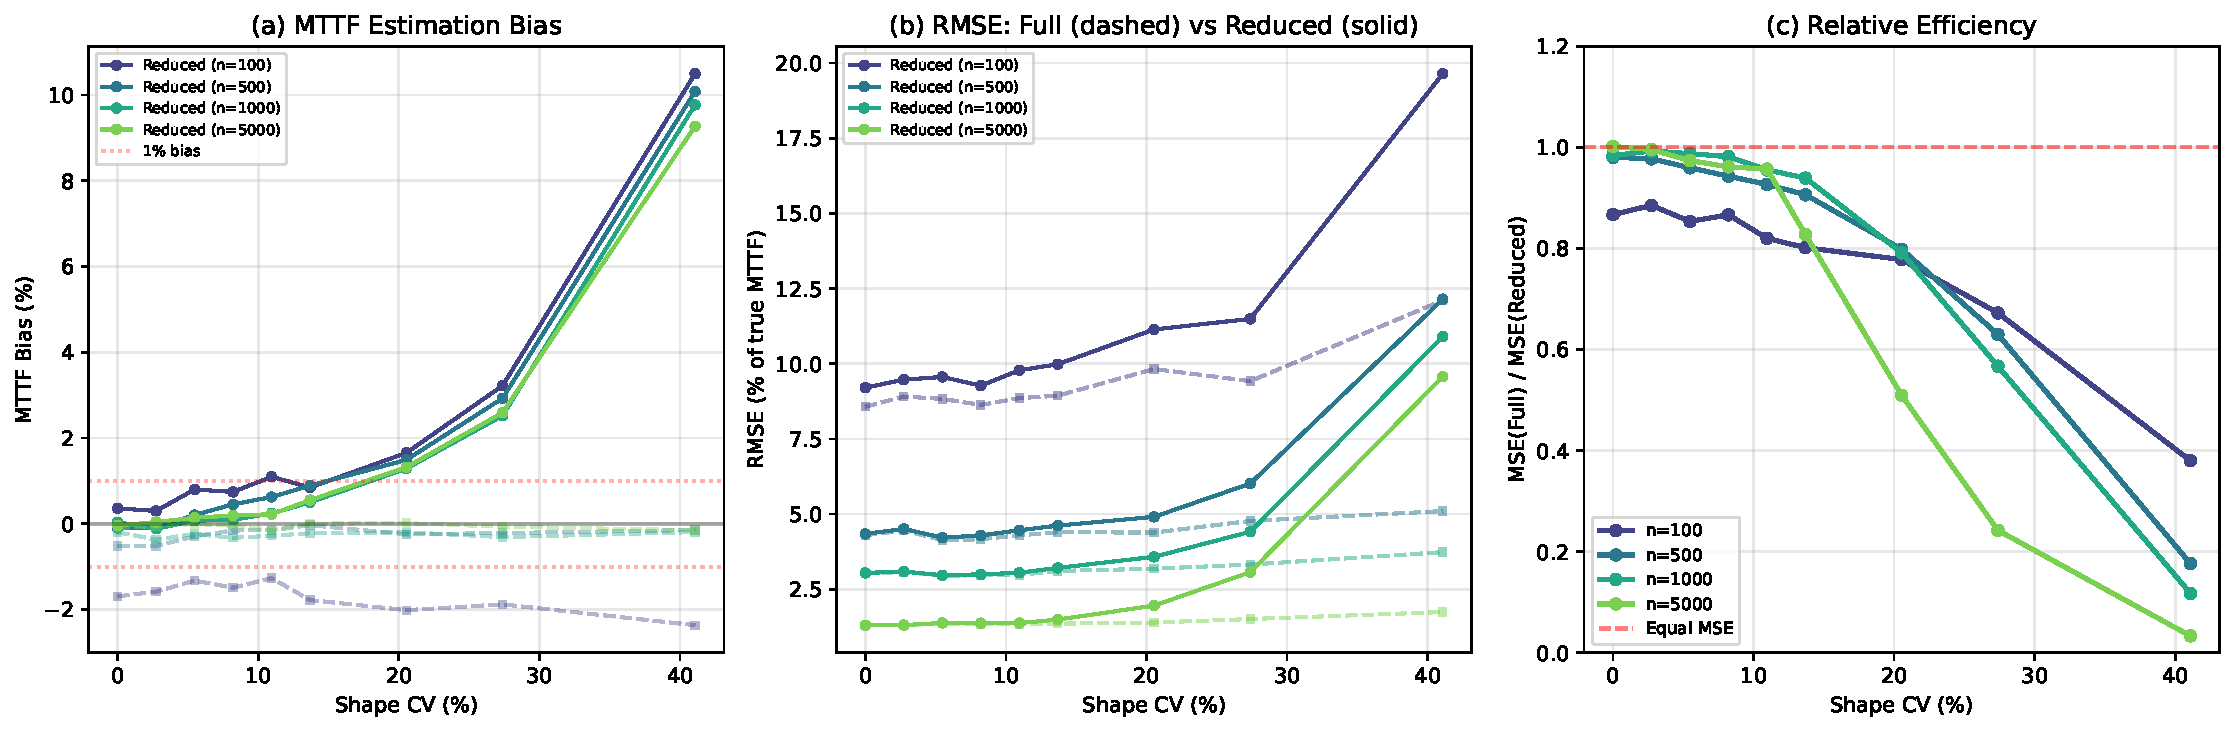
\includegraphics[width=0.85\textwidth]{image/consequence_analysis.pdf}
\caption{Consequence analysis. (a)~MTTF bias: dashed lines show the full model (near zero at all CVs), solid lines show the reduced model (growing with CV). (b)~RMSE comparison as percentage of true MTTF. (c)~Relative efficiency: the full model has lower MSE at all CVs, increasingly so for higher CV. (d)~Consequence vs detectability: the LRT rejects the reduced model only when bias becomes large.}
\label{fig:consequence}
\end{figure}

Three patterns emerge. First, the reduced model's MTTF bias is remarkably small: below 1\% through shape CV $\approx 14\%$ at $n \geq 500$, and the 1\% threshold is not crossed until CV $\approx 20\%$ (bias $= 1.5\%$). Only at CV $> 27\%$ does the bias exceed 2.5\%. Second, the bias is almost entirely positive---the reduced model systematically overestimates MTTF because the common-shape fit overestimates the weaker components. Third, the bias is largely independent of sample size: a 50-fold increase from $n = 100$ to $n = 5000$ changes the bias at CV $\approx 27\%$ from $+3.2\%$ to $+2.6\%$, confirming that this is a specification bias, not a finite-sample artifact.

The reliability function $R(t)$ evaluated at the system MTTF shows analogous behavior. The reduced model's $R(\text{MTTF})$ bias is below 0.5\% for CV $\leq 10\%$ and grows to approximately $-4\%$ at CV $= 30\%$. The negative sign indicates that the reduced model underestimates reliability at the MTTF, consistent with the Weibull closure property forcing a compromise shape.

\subsection{Discussion}

A surprising finding is that the full model has lower MSE than the reduced model at practical sample sizes ($n \leq 1000$)---even when the reduced model is correctly specified (CV $= 0$). A bias-variance decomposition (Figure~\ref{fig:mse-decomp}) reveals the mechanism: at $n = 100$ and CV $= 0$, the full model's MTTF variance (348) is substantially lower than the reduced model's (417), despite having more parameters. The traditional argument that parsimony reduces estimator variance holds for the shape parameters themselves, but the system MTTF is a nonlinear functional $\text{MTTF} = \int_0^\infty \exp\{-\sum_j (t/\lambda_j)^{k_j}\}\, dt$ that can amplify variance differently under constrained versus unconstrained parameterizations \cite{White-1982}. The constraint $k_1 = \cdots = k_m$ forces all shape estimation error into a single degree of freedom, which then propagates through the nonlinear MTTF integral with greater amplification than the distributed errors of the unconstrained estimator. At $n = 5000$ the two models achieve approximately equal MSE as the variance contribution diminishes.

This has a practical implication: \emph{the traditional argument for the reduced model---lower variance from fewer parameters---does not hold for system-level predictions}. The case for the common-shape model rests instead on interpretability, the Weibull closure property, and the empirical observation that its predictions are accurate enough for engineering use when shape heterogeneity is modest.

Figure~\ref{fig:consequence}(d) reveals the relationship between detectability and consequence: the LRT rejection rate and the reduced model's bias both increase with CV, but they track different curves. At $n = 500$: at CV $\approx 14\%$, the LRT rejection rate is 37\% while the MTTF bias is only 0.9\%---the test has substantial probability of rejecting a model whose predictions are adequate. At CV $\approx 21\%$, the test rejects 97\% of the time and the bias is 1.5\%. At CV $\approx 27\%$, the bias reaches 2.9\%, warranting the switch to the full model.

\begin{figure}[htbp]
\centering
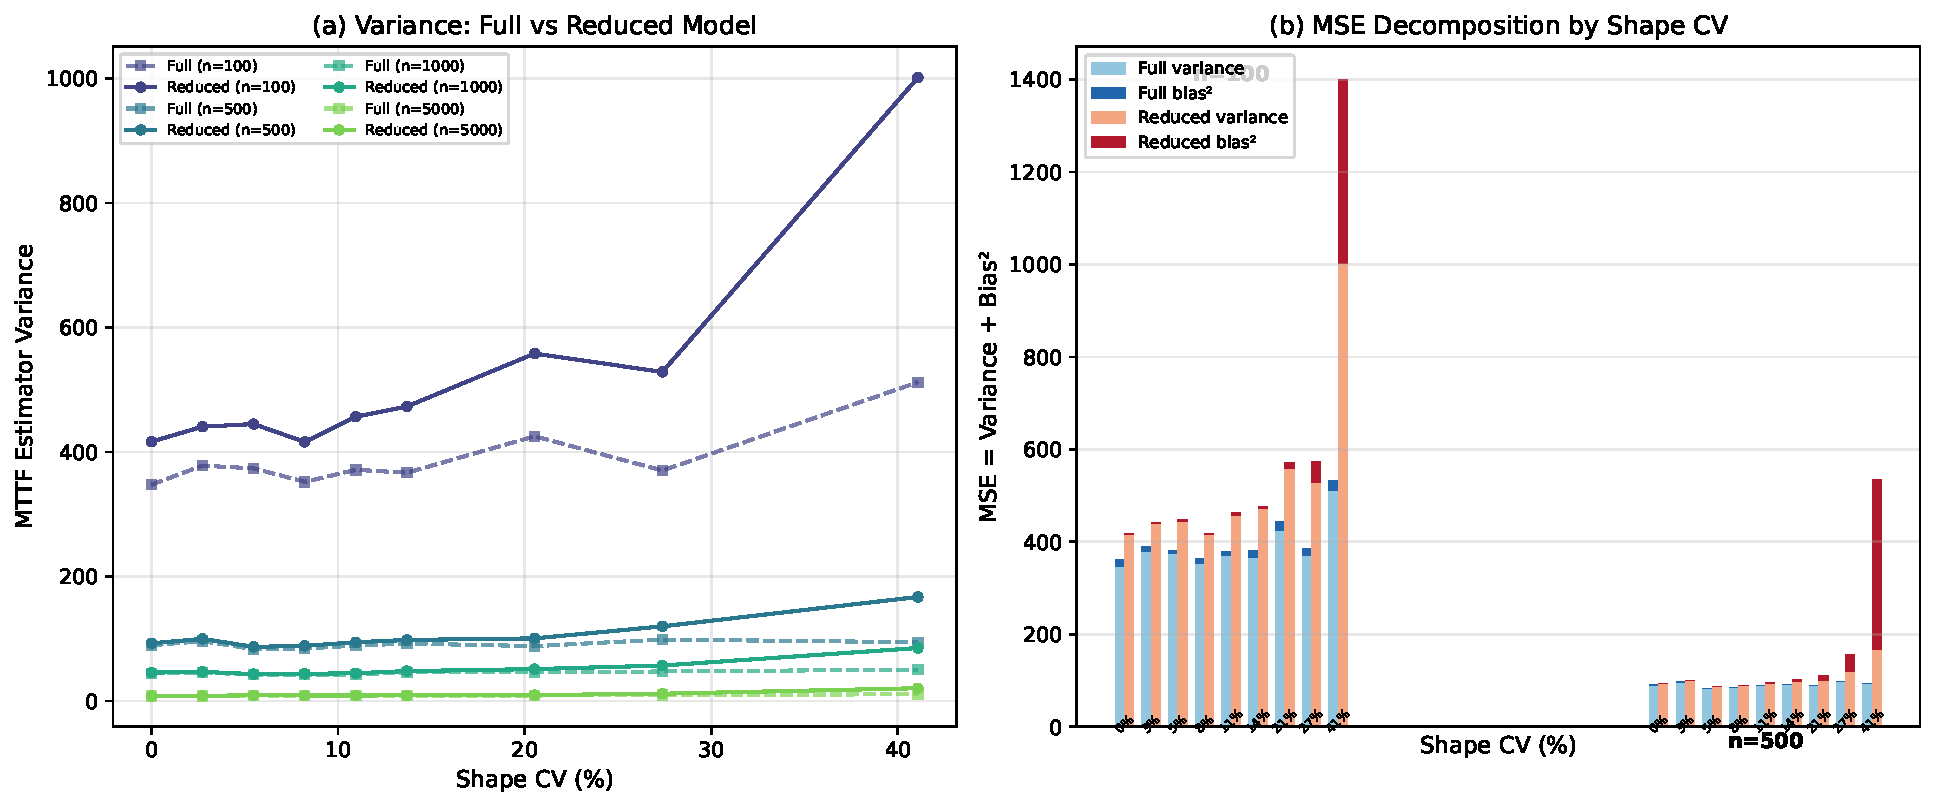
\includegraphics[width=0.85\textwidth]{image/mse_decomposition.pdf}
\caption{Bias-variance decomposition of MTTF MSE. (a)~Variance comparison: the full model has lower MTTF variance than the reduced model at all CVs, despite having more parameters. (b)~MSE decomposition: the reduced model's MSE is dominated by variance at low CV, then by bias$^2$ at high CV.}
\label{fig:mse-decomp}
\end{figure}

%% =========================================================================
\section{Likelihood Ratio Testing}
\label{sec:lrt}

The consequence analysis shows \emph{when misspecification matters} for predictions. This section addresses a complementary question: \emph{when can the data distinguish} between the full and reduced models? We employ the likelihood ratio test (LRT) with statistic
\begin{equation}
\Lambda = -2 (\ell(\hat{\v\theta}_R) - \ell(\hat{\v\theta}_F)),
\end{equation}
which is asymptotically $\chi^2_{m-1}$ under the null hypothesis $H_0: k_1 = \cdots = k_m$ \cite{wilks1938}.

\subsection{Type I Error Validation}

Table~\ref{tab:type1-error} presents rejection rates at $\alpha = 0.05$ under perfect homogeneity ($\text{CV}_k = 0$). All rates are consistent with the nominal level, confirming the $\chi^2_{m-1}$ approximation. The $\chi^2$ approximation is asymptotic; at $n = 100$ with $m - 1 = 4$ degrees of freedom, finite-sample deviations may occur, though our Type~I error validation confirms adequate calibration across all sample sizes tested.

\begin{table}[htbp]
\centering
\caption{LRT Type I Error Rate Under Perfect Homogeneity ($\text{CV}_k = 0$)}
\label{tab:type1-error}
\begin{tabular}{cccc}
\hline
Sample Size $n$ & Rejection Rate & 95\% CI & Status \\
\hline
100 & 0.054 & [0.037, 0.077] & OK \\
500 & 0.056 & [0.039, 0.080] & OK \\
1000 & 0.046 & [0.031, 0.068] & OK \\
5000 & 0.068 & [0.049, 0.094] & OK \\
10000 & 0.046 & [0.031, 0.068] & OK \\
\hline
\end{tabular}
\end{table}

\subsection{Power Analysis}

Figure~\ref{fig:lrt-power-curves} and Table~\ref{tab:power-by-cv} present the LRT rejection rate (power) as a function of shape CV for different sample sizes.

\begin{figure}[htbp]
\centering

\includegraphics[width=0.85\textwidth]{image/lrt_divergence_analysis.pdf}
\caption{LRT power as a function of shape parameter divergence. Top left: Power curves by sample size. Top right: Heatmap of rejection rates. Bottom left: Type I error region (low CV). Bottom right: Power curves (clean view, no CIs).}
\label{fig:lrt-power-curves}
\end{figure}

\begin{table}[htbp]
\centering
\caption{LRT Rejection Rate by Divergence Level and Sample Size}
\label{tab:power-by-cv}
\small
\begin{tabular}{cccccc}
\hline
CV (\%) & $n = 100$ & $n = 500$ & $n = 1000$ & $n = 5000$ & $n = 10000$ \\
\hline
0.0 & 0.054 & 0.056 & 0.046 & 0.068 & 0.046 \\
2.7 & 0.048 & 0.062 & 0.052 & 0.186 & 0.268 \\
5.5 & 0.075 & 0.072 & 0.130 & 0.541 & 0.887 \\
8.2 & 0.074 & 0.126 & 0.266 & 0.936 & 0.996 \\
11.0 & 0.088 & 0.252 & 0.494 & 0.996 & 1.000 \\
\hline
\end{tabular}
\end{table}

The key observation: at CV $\leq 5\%$, the LRT has almost no power at practical sample sizes ($n \leq 1000$). Even at $n = 10{,}000$, the rejection rate at CV $= 2.7\%$ is only 27\%. Combined with the consequence analysis showing that prediction bias is negligible in this regime, the case for the common-shape model is strong.

\subsection{Factors Affecting Power}

We examined how masking probability, censoring level, and system complexity affect LRT performance. These simulations used the baseline well-designed system (CV $\approx 4\%$).

\paragraph{Masking probability.}
Figure~\ref{fig:lrt-vary-p} shows that higher masking reduces power. At $n = 5000$, the rejection rate drops from 48\% at $p = 0.05$ to 8\% at $p = 0.70$. Masking reduces the information about which component caused each failure.

\begin{figure}[htbp]
\centering

\includegraphics[width=0.8\textwidth]{image/lrt_vary_p_rejection_rate.pdf}
\caption{Effect of masking probability on LRT rejection rate.}
\label{fig:lrt-vary-p}
\end{figure}

\paragraph{Censoring level.}
Figure~\ref{fig:lrt-vary-q} shows that heavier censoring (lower $q$) reduces power. At $n = 5000$, the rejection rate increases from 17\% at $q = 0.5$ to 43\% at $q = 1.0$. Censored observations provide reliability information but no failure attribution.

\begin{figure}[htbp]
\centering

\includegraphics[width=0.8\textwidth]{image/lrt_vary_q_rejection_rate.pdf}
\caption{Effect of censoring quantile on LRT rejection rate.}
\label{fig:lrt-vary-q}
\end{figure}

\paragraph{System complexity.}
Figure~\ref{fig:lrt-vary-m} shows that power decreases with the number of components. At $n = 5000$, the rejection rate drops from 77\% at $m = 2$ to 16\% at $m = 8$. The LRT has $m-1$ degrees of freedom, so larger systems have higher critical values, and failure information is distributed across more parameters. Note that the shape CV decreases slightly from 5.5\% ($m=2$) to 3.5\% ($m=8$) in our design, which partially confounds the effect of system complexity with reduced heterogeneity.

\begin{figure}[htbp]
\centering

\includegraphics[width=0.85\textwidth]{image/lrt_vary_m_rejection_rate.pdf}
\caption{Effect of number of components on LRT rejection rate.}
\label{fig:lrt-vary-m}
\end{figure}

Of the data quality factors, masking has the larger impact: increasing masking probability from 0.05 to 0.70 reduces power by a factor of 6, while removing censoring entirely increases power by a factor of 2.5. Importantly, neither factor inflates the Type~I error rate---the test remains well-calibrated throughout.

\subsection{Comparison with Information Criteria}

We compare the LRT with AIC \cite{akaike1974} and BIC \cite{schwarz1978}. For two competing models with log-likelihoods $\ell_F$ ($2m$ parameters) and $\ell_R$ ($m+1$ parameters):
\begin{align}
\text{AIC} &= -2\ell + 2k, \\
\text{BIC} &= -2\ell + k \ln n,
\end{align}
where $k$ is the number of model parameters ($2m$ for the full model, $m+1$ for the reduced model).

\begin{figure}[htbp]
\centering
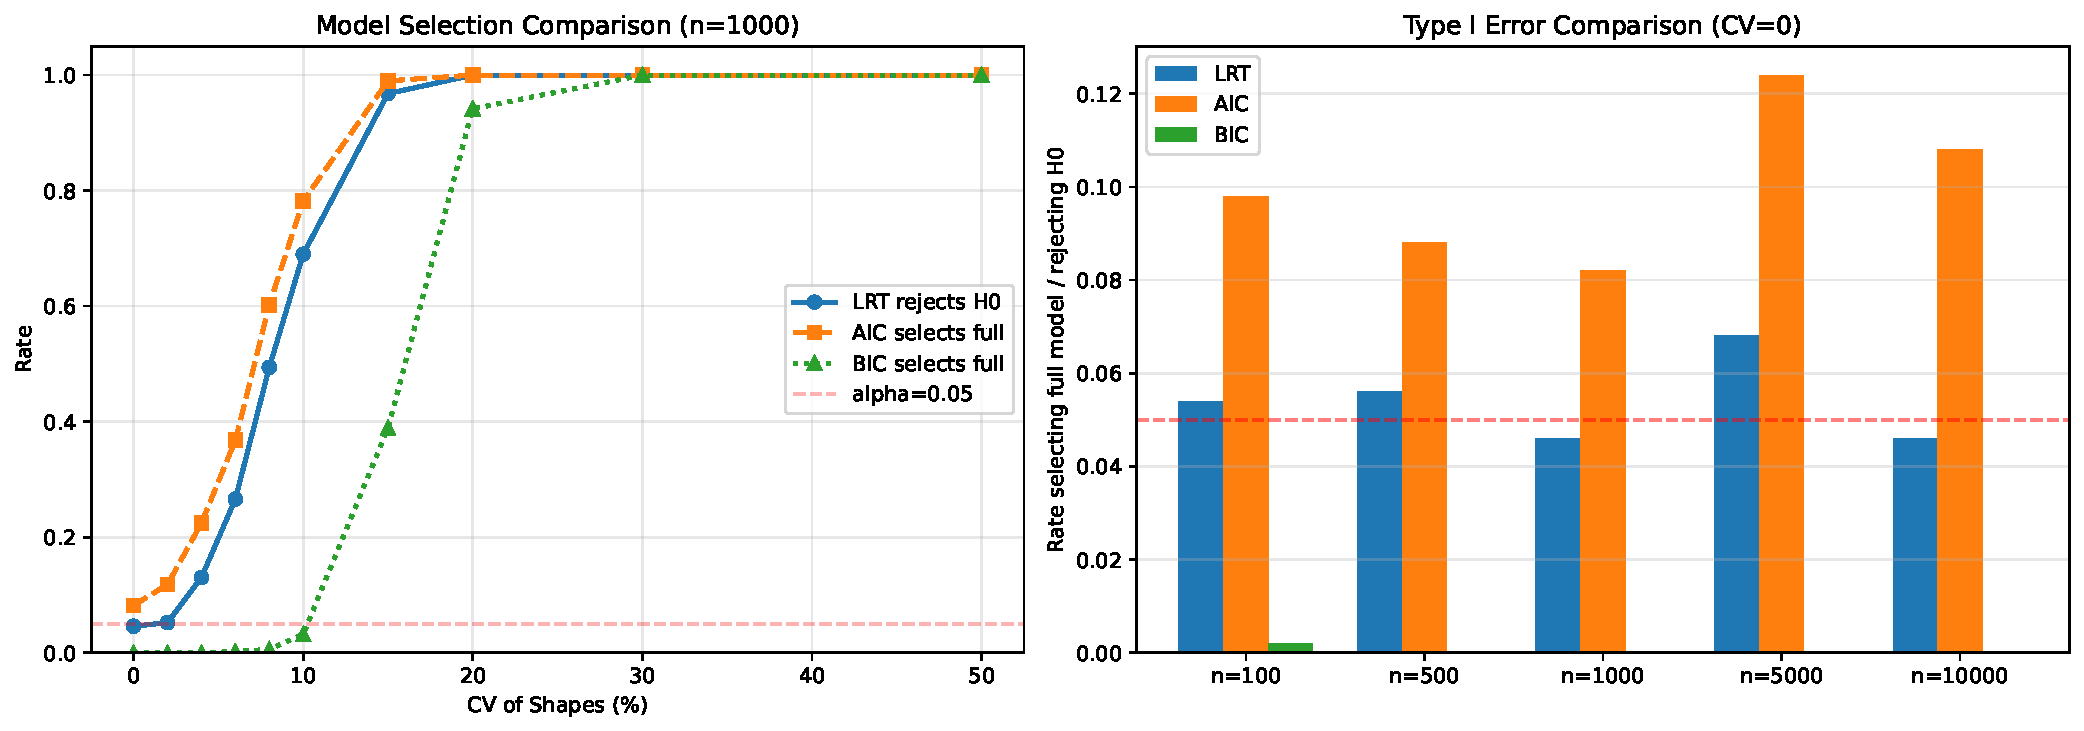
\includegraphics[width=0.85\textwidth]{image/lrt_vs_aic_bic_divergence.pdf}
\caption{Model selection rates for LRT ($\alpha = 0.05$), AIC, and BIC vs shape CV.}
\label{fig:lrt-vs-aic-bic}
\end{figure}

Figure~\ref{fig:lrt-vs-aic-bic} and Table~\ref{tab:type1-criteria} summarize the comparison. Note that AIC and BIC are model selection criteria rather than hypothesis tests; the ``Type~I error'' rates reported here represent the proportion of times each criterion selects the full model under perfect homogeneity, enabling a calibration comparison but not a direct power comparison. The LRT is well-calibrated (4.6--6.8\%), AIC is liberal (8.2--12.4\%, roughly $2\times$ the nominal rate), and BIC is over-conservative (0--0.2\%). For formal hypothesis testing of shape homogeneity, the LRT provides the best-calibrated Type~I error while maintaining good power. AIC may be useful for exploratory analysis where false positives are less costly than missed heterogeneity. BIC's conservatism makes it unsuitable for detecting the subtle heterogeneity characteristic of well-designed systems.

\begin{table}[htbp]
\centering
\caption{Type~I Error Comparison Under Perfect Homogeneity ($\text{CV}_k = 0$)}
\label{tab:type1-criteria}
\small
\begin{tabular}{lcc}
\hline
Criterion & Selection Rate Range & Behavior \\
\hline
LRT ($\alpha = 0.05$) & 4.6--6.8\% & Well-calibrated \\
AIC & 8.2--12.4\% & Liberal (${\approx}\,2{\times}$ nominal) \\
BIC & 0--0.2\% & Over-conservative \\
\hline
\end{tabular}
\end{table}

%% =========================================================================
\section{Adaptive Model Selection}
\label{sec:adaptive}

The preceding sections establish \emph{when} the common-shape model is adequate (consequence analysis) and \emph{whether} the data can distinguish it from the full model (LRT). This section addresses the practical question: given data from an unknown system, how should a practitioner choose between models?

\subsection{Procedure}

We evaluate a natural LRT-based adaptive procedure:
\begin{enumerate}
\item Fit the full model ($2m$ parameters) to obtain $\hat{\v\theta}_F$.
\item Fit the reduced model ($m+1$ parameters) to obtain $\hat{\v\theta}_R$.
\item Compute the LRT statistic $\Lambda = -2(\ell(\hat{\v\theta}_R) - \ell(\hat{\v\theta}_F))$.
\item If $\Lambda < \chi^2_{m-1, 1-\alpha}$ (i.e., $p > \alpha$), use the reduced model; otherwise use the full model.
\end{enumerate}

This procedure inherits the well-calibrated Type~I error of the LRT (Table~\ref{tab:type1-error}): under the null, the reduced model is selected with probability $1 - \alpha$.

We also compare with a simpler CV-based approach: fit the full model, compute $\widehat{\text{CV}}_k = \text{sd}(\hat{k}_1, \ldots, \hat{k}_m) / \text{mean}(\hat{k}_1, \ldots, \hat{k}_m)$, and select the reduced model if $\widehat{\text{CV}}_k < \tau$ for a threshold $\tau$.

\subsection{Simulation Design}

We compare four strategies:
\begin{enumerate}
\item \textbf{Always-full}: use full model estimates regardless
\item \textbf{Always-reduced}: use reduced model estimates regardless
\item \textbf{Adaptive (LRT)}: select model via the LRT at $\alpha = 0.05$
\item \textbf{Adaptive (CV)}: select model via estimated CV threshold
\end{enumerate}

We evaluate on MTTF estimation accuracy (MSE, bias) across shape CV from 0 to 20\% and sample sizes $n \in \{100, 500, 1000\}$, with 500 replications per condition. Non-convergent fits are excluded (typically $< 2\%$ of replications).

\subsection{Results}

Table~\ref{tab:adaptive} presents the RMSE of each strategy as a percentage of the true system MTTF, along with the fraction of replications where the LRT-based adaptive procedure selects the reduced model. Figure~\ref{fig:adaptive} provides the corresponding visualization.

\begin{table}[htbp]
\centering
\caption{Adaptive Model Selection: RMSE (\% of True MTTF) and Selection Rate}
\label{tab:adaptive}
\small
\begin{tabular}{cccccc}
\hline
CV (\%) & $n$ & Full & Reduced & Adaptive & Sel.~Red. (\%) \\
\hline
0.0 & 100 & 9.3 & 10.1 & 10.0 & 93 \\
    & 500 & 4.6 & 4.7 & 4.7 & 95 \\
    & 1000 & 3.0 & 3.0 & 3.0 & 94 \\
\hline
5.5 & 100 & 9.3 & 10.1 & 10.1 & 95 \\
    & 500 & 4.1 & 4.2 & 4.2 & 92 \\
    & 1000 & 3.0 & 3.0 & 3.1 & 89 \\
\hline
13.7 & 100 & 9.5 & 10.4 & 10.3 & 89 \\
     & 500 & 4.3 & 4.5 & 4.4 & 60 \\
     & 1000 & 3.0 & 3.2 & 3.0 & 30 \\
\hline
20.5 & 100 & 9.5 & 10.7 & 10.4 & 83 \\
     & 500 & 4.4 & 4.9 & 4.5 & 21 \\
     & 1000 & 3.2 & 3.6 & 3.2 & 1 \\
\hline
27.4 & 100 & 9.9 & 12.8 & 11.6 & 65 \\
     & 500 & 4.6 & 5.6 & 4.7 & 1 \\
     & 1000 & 3.3 & 4.4 & 3.3 & 0 \\
\hline
\end{tabular}
\end{table}

\begin{figure}[htbp]
\centering
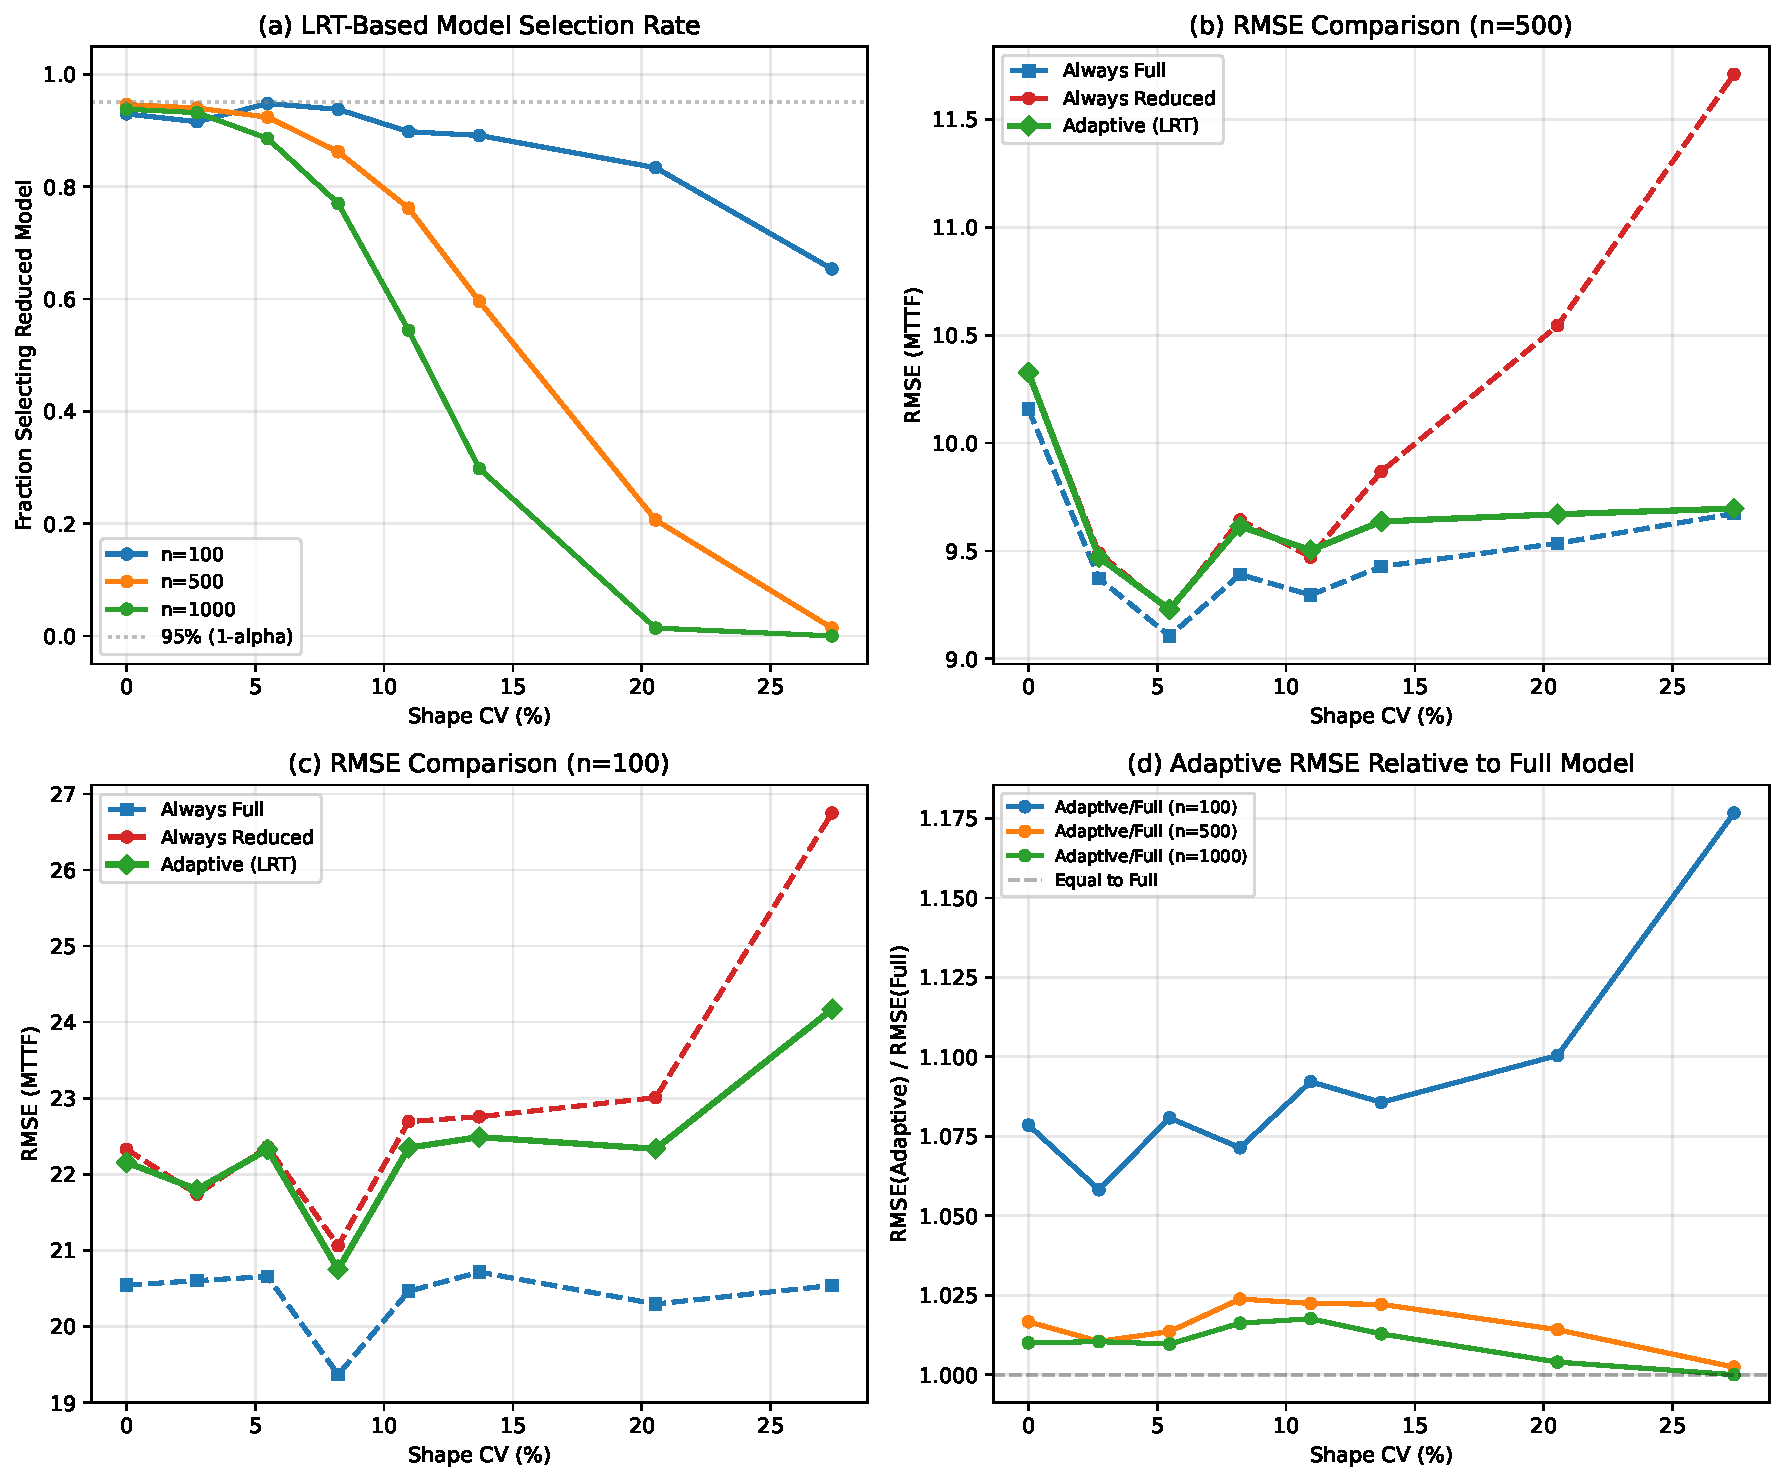
\includegraphics[width=0.85\textwidth]{image/adaptive_selection.pdf}
\caption{Adaptive model selection. (a)~Selection rate: the LRT correctly selects the reduced model near 95\% at CV~$= 0$ and transitions smoothly to the full model as CV increases, with the transition point shifting left with sample size. (b)--(c)~RMSE comparison at $n = 500$ and $n = 100$: the adaptive procedure (green) tracks the better of the two static strategies across all CVs. (d)~Relative RMSE: the adaptive procedure's overhead ranges from 8--18\% at $n = 100$ and is under 2.5\% at $n = 500$.}
\label{fig:adaptive}
\end{figure}

The adaptive procedure exhibits three regimes. At \textbf{low CV} ($\leq 5\%$), the procedure selects the reduced model in $> 90\%$ of replications across all sample sizes, achieving RMSE comparable to the always-reduced strategy. At \textbf{moderate CV} (5--14\%), the selection rate depends strongly on sample size: at $n = 100$ the procedure still selects reduced $\sim 90\%$ of the time (because the LRT lacks power), while at $n = 1000$ the selection rate drops to 30\% at CV $\approx 14\%$. At \textbf{high CV} ($> 20\%$), the procedure overwhelmingly selects the full model at $n \geq 500$, protecting against the large bias of the reduced model.

The RMSE overhead of the adaptive procedure relative to the always-full strategy is at most 2.4\% at $n = 500$ and converges to zero at large $n$ and high CV. At $n = 100$, the overhead ranges from 8\% to 18\%, with the largest values occurring at high CV where the reduced model has substantial MTTF bias. However, even this ``failure'' is partially benign: the consequence analysis (Table~\ref{tab:consequence}) shows that the reduced model's bias remains moderate at the CVs where the LRT lacks power to reject it.

\subsection{Discussion}

The adaptive procedure succeeds because of a fortuitous alignment: the LRT has low power precisely where the consequence of misspecification is small, and high power where the consequence is large. At $n = 500$ and CV $\approx 14\%$, the adaptive procedure selects the reduced model 60\% of the time; the bias of the reduced model at this CV is only 0.9\%, so these ``incorrect'' selections carry negligible penalty. At CV $\approx 21\%$, the procedure selects the full model 79\% of the time, and at CV $\approx 27\%$ it selects the full model 99\% of the time, avoiding the 2.9\% bias.

The CV-based adaptive procedure performs similarly to the LRT-based approach but requires choosing a threshold $\tau$ that does not automatically adapt to sample size or data quality. The LRT is preferred because its critical value incorporates the degrees of freedom and sample size naturally.

From a practical standpoint, the adaptive procedure adds no cost beyond fitting both models. Since both fits are required to compute the LRT statistic, the procedure is a free byproduct of the testing framework described in Section~\ref{sec:lrt}.

%% =========================================================================
\section{Conclusion}
\label{sec:conclusion}

This paper addressed a fundamental question in reliability engineering: when can practitioners safely simplify a Weibull series system model by assuming common component shapes? The answer is structured around a quantitative alignment between prediction consequence and statistical detectability.

\paragraph{Bias and power are quantitatively aligned.}
The common-shape model's MTTF bias grows super-linearly with shape heterogeneity---remaining below 1\% through CV $\approx 15\%$---while the LRT's power grows super-linearly. The practical consequence: the test lacks power precisely where misspecification is harmless for engineering decisions, and has high power precisely where the bias warrants switching to the full model. An adaptive LRT-based procedure exploits this alignment, achieving RMSE within 2.5\% of the always-full strategy at $n \geq 500$ while selecting the simpler model over 90\% of the time when the data support it.

\paragraph{The traditional argument for the reduced model does not hold.}
Surprisingly, a bias-variance decomposition (Figure~\ref{fig:mse-decomp}) reveals that the full model has lower MTTF variance than the reduced model even when the reduced model is correctly specified (CV $= 0$). The constraint $k_1 = \cdots = k_m$ forces all shape estimation error into a single degree of freedom, amplifying its propagation through the nonlinear MTTF integral. The case for the common-shape model rests instead on interpretability, the Weibull closure property, and the empirical demonstration that its predictions are engineering-adequate across a broad range of shape heterogeneity.

\paragraph{The LRT is well-calibrated; information criteria are not.}
Among model selection criteria, the LRT provides well-calibrated Type~I error (4.6--6.8\% at nominal $\alpha = 0.05$), while AIC is liberal (${\approx}2\times$ nominal false positive rate) and BIC is over-conservative (${\leq}0.2\%$). The LRT has negligible power at CV below 5\% for $n \leq 1{,}000$; even at $n = 10{,}000$, the rejection rate at CV $\approx 3\%$ is only 27\%.

\paragraph{Data quality effects.}
Higher masking probabilities and heavier censoring reduce the power of all model selection methods by diminishing the information available for discriminating between models, but they do not inflate the Type~I error rate. Of the two, masking has the larger impact (6$\times$ reduction in power from $p = 0.05$ to $p = 0.70$, vs 2.5$\times$ from $q = 0.50$ to $q = 1.00$).

\paragraph{Limitations.}
Our simulations use uniformly spaced shapes about a common mean. Real systems may exhibit asymmetric or clustered heterogeneity patterns. The single baseline system (5 components, moderate masking and censoring) may not capture all configurations of practical interest.

\paragraph{Future directions.}
Three extensions merit investigation. First, the common-shape assumption could be tested for non-Weibull distributions where analogous closure properties may or may not hold. Second, optimal experimental design for model selection would provide guidance on sample size and diagnostic effort. Third, extending to parallel and $k$-out-of-$n$ configurations would broaden applicability.

\appendix

\section{MLE Sensitivity to System Design Perturbations}
\label{app:sensitivity}

This appendix examines how deviations from the baseline system configuration affect MLE performance, motivating the model selection analysis in the main text.

\subsection{Effect of Scale Parameter Perturbation}

Figure~\ref{fig:mttf-vs-ci} shows the effect of varying component 3's scale parameter $\lambda_3$ (mapped to MTTF$_3$) on MLE dispersion, bias, and coverage probability.

\begin{figure}[htbp]
\centering
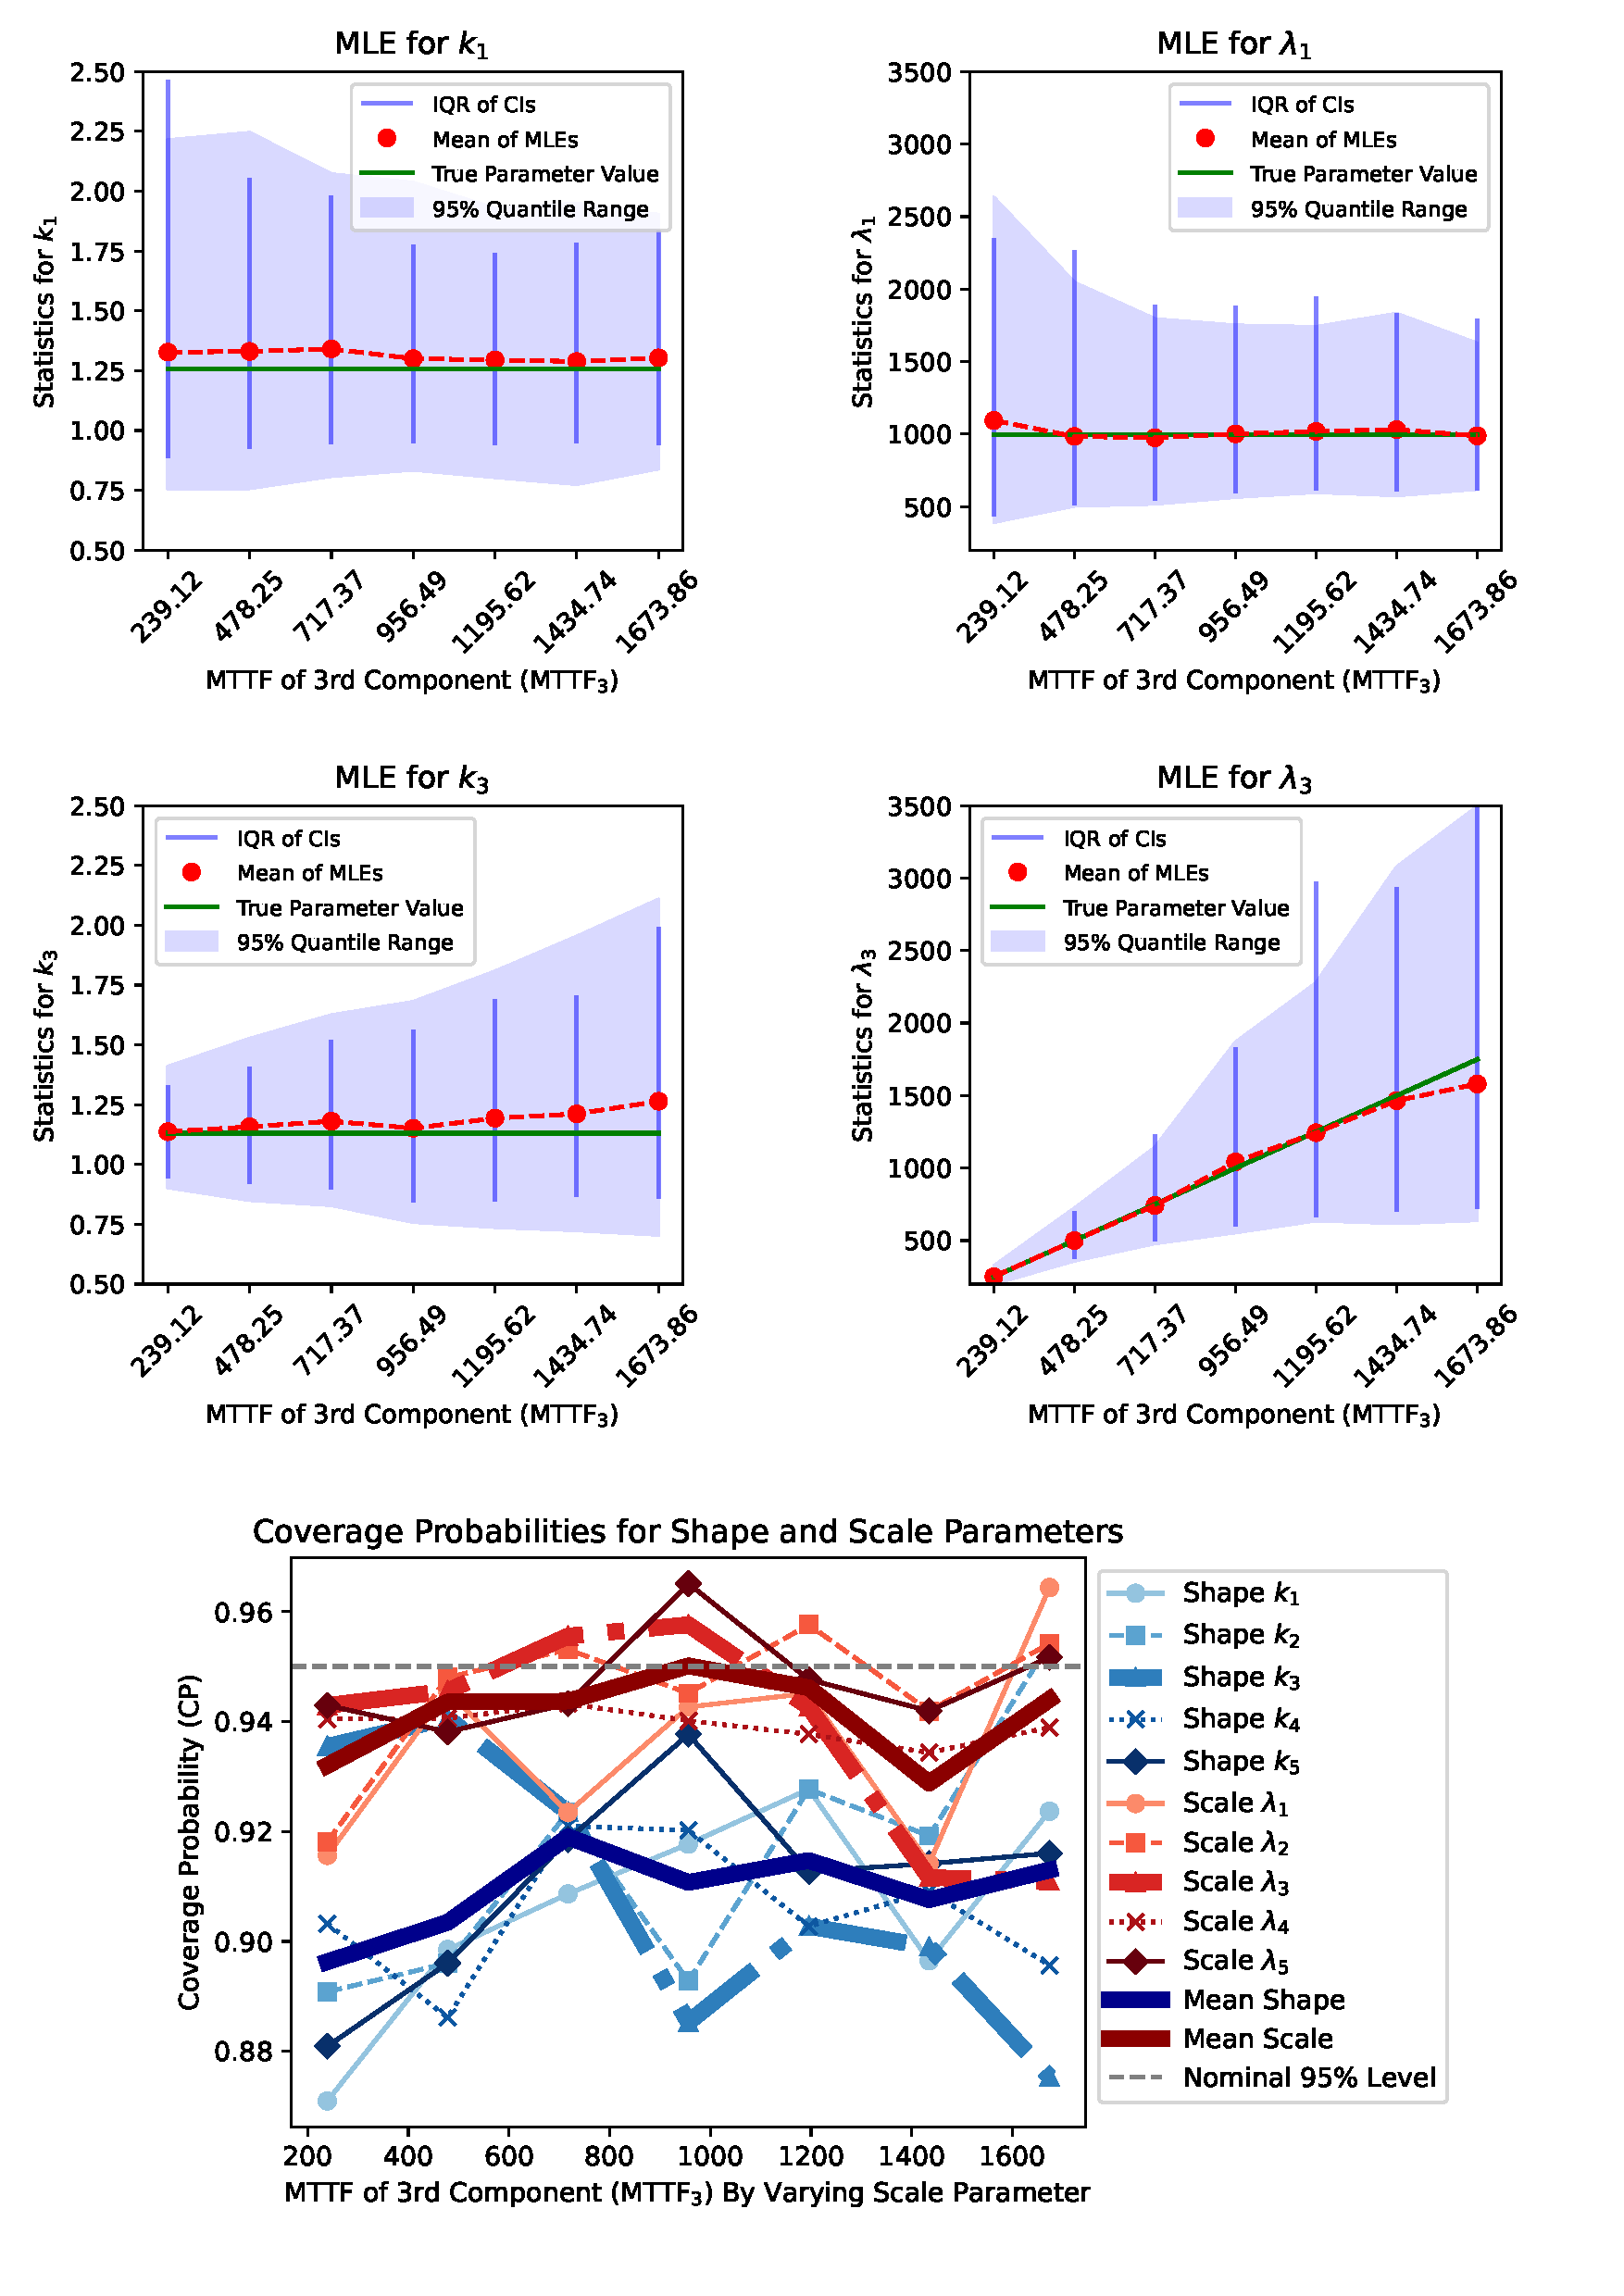
\includegraphics[width=0.8\textwidth]{image/5_system_mttf3_by_scale3.pdf}
\caption{MLE performance vs MTTF of component 3 (by varying scale $\lambda_3$). Components with smaller MTTF cause more system failures and are estimated more precisely.}
\label{fig:mttf-vs-ci}
\end{figure}

As component 3's MTTF decreases below other components, it causes more system failures, providing more information for its own parameter estimation (lower dispersion, better coverage) at the expense of other components.

\subsection{Effect of Shape Parameter Perturbation}

Figure~\ref{fig:prob3-vs-mle} shows the effect of varying component 3's shape parameter $k_3$ on MLE performance. The relationship between $k_3$ and the probability of component 3 causing system failure is complex: components with $k < 1$ exhibit high early hazard and dominate system failures despite having higher MTTFs.

\begin{figure}[htbp]
\centering
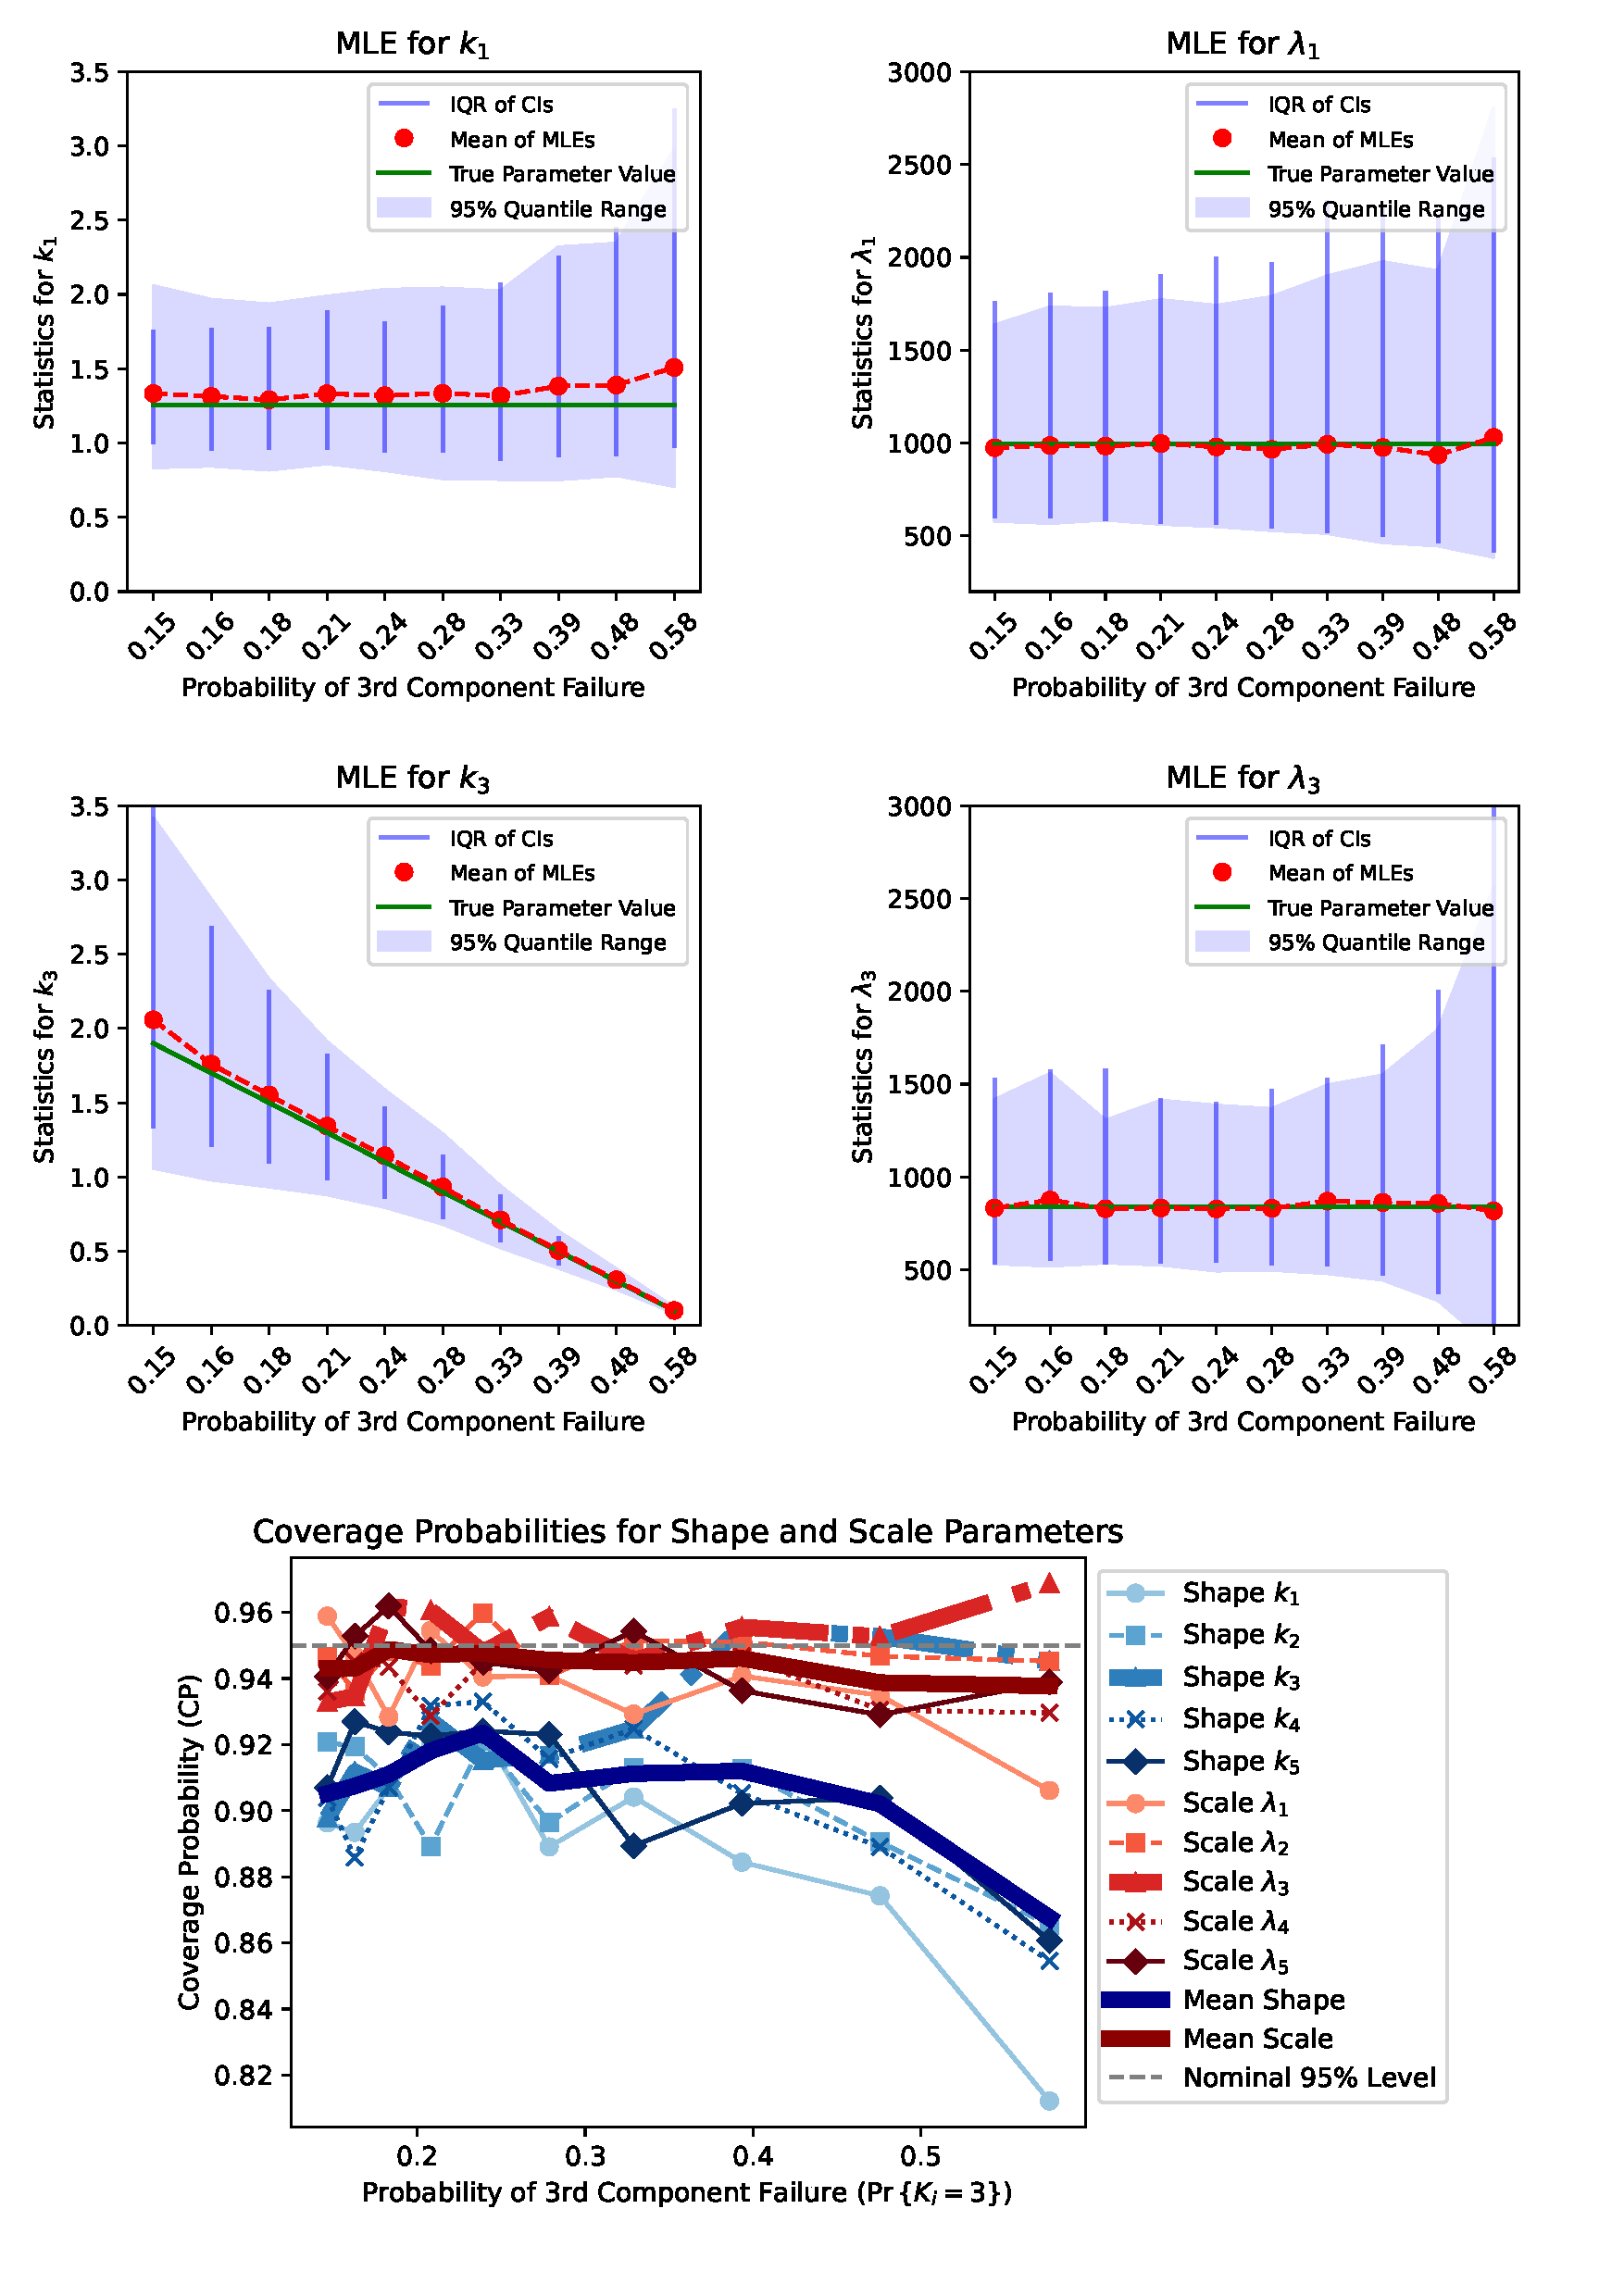
\includegraphics[width=0.85\textwidth]{image/5_system_shape3_fig.pdf}
\caption{MLE performance vs probability of component 3 failure (by varying shape $k_3$). Shape parameters are harder to estimate than scale parameters, particularly when failure probability is low.}
\label{fig:prob3-vs-mle}
\end{figure}

These results confirm that (1) shape parameters are inherently harder to estimate than scale parameters, and (2) estimator precision depends strongly on component failure probability. Both observations motivate the common-shape model: by pooling shape information across components, the reduced model effectively increases the sample size for the shared shape parameter.

\section{Ideal Case Analysis}
\label{app:ideal-case}

Figure~\ref{fig:ideal-case} examines MLE behavior under ideal conditions---no masking ($p = 0$) and no censoring ($q = 1$)---using a 2-component system with $n = 100$. Even with perfect information, shape parameter estimates exhibit bias for components with low failure probabilities, confirming that estimation difficulty is inherent to series systems, not solely a consequence of masked or censored data.

\begin{figure}[htbp]
\centering
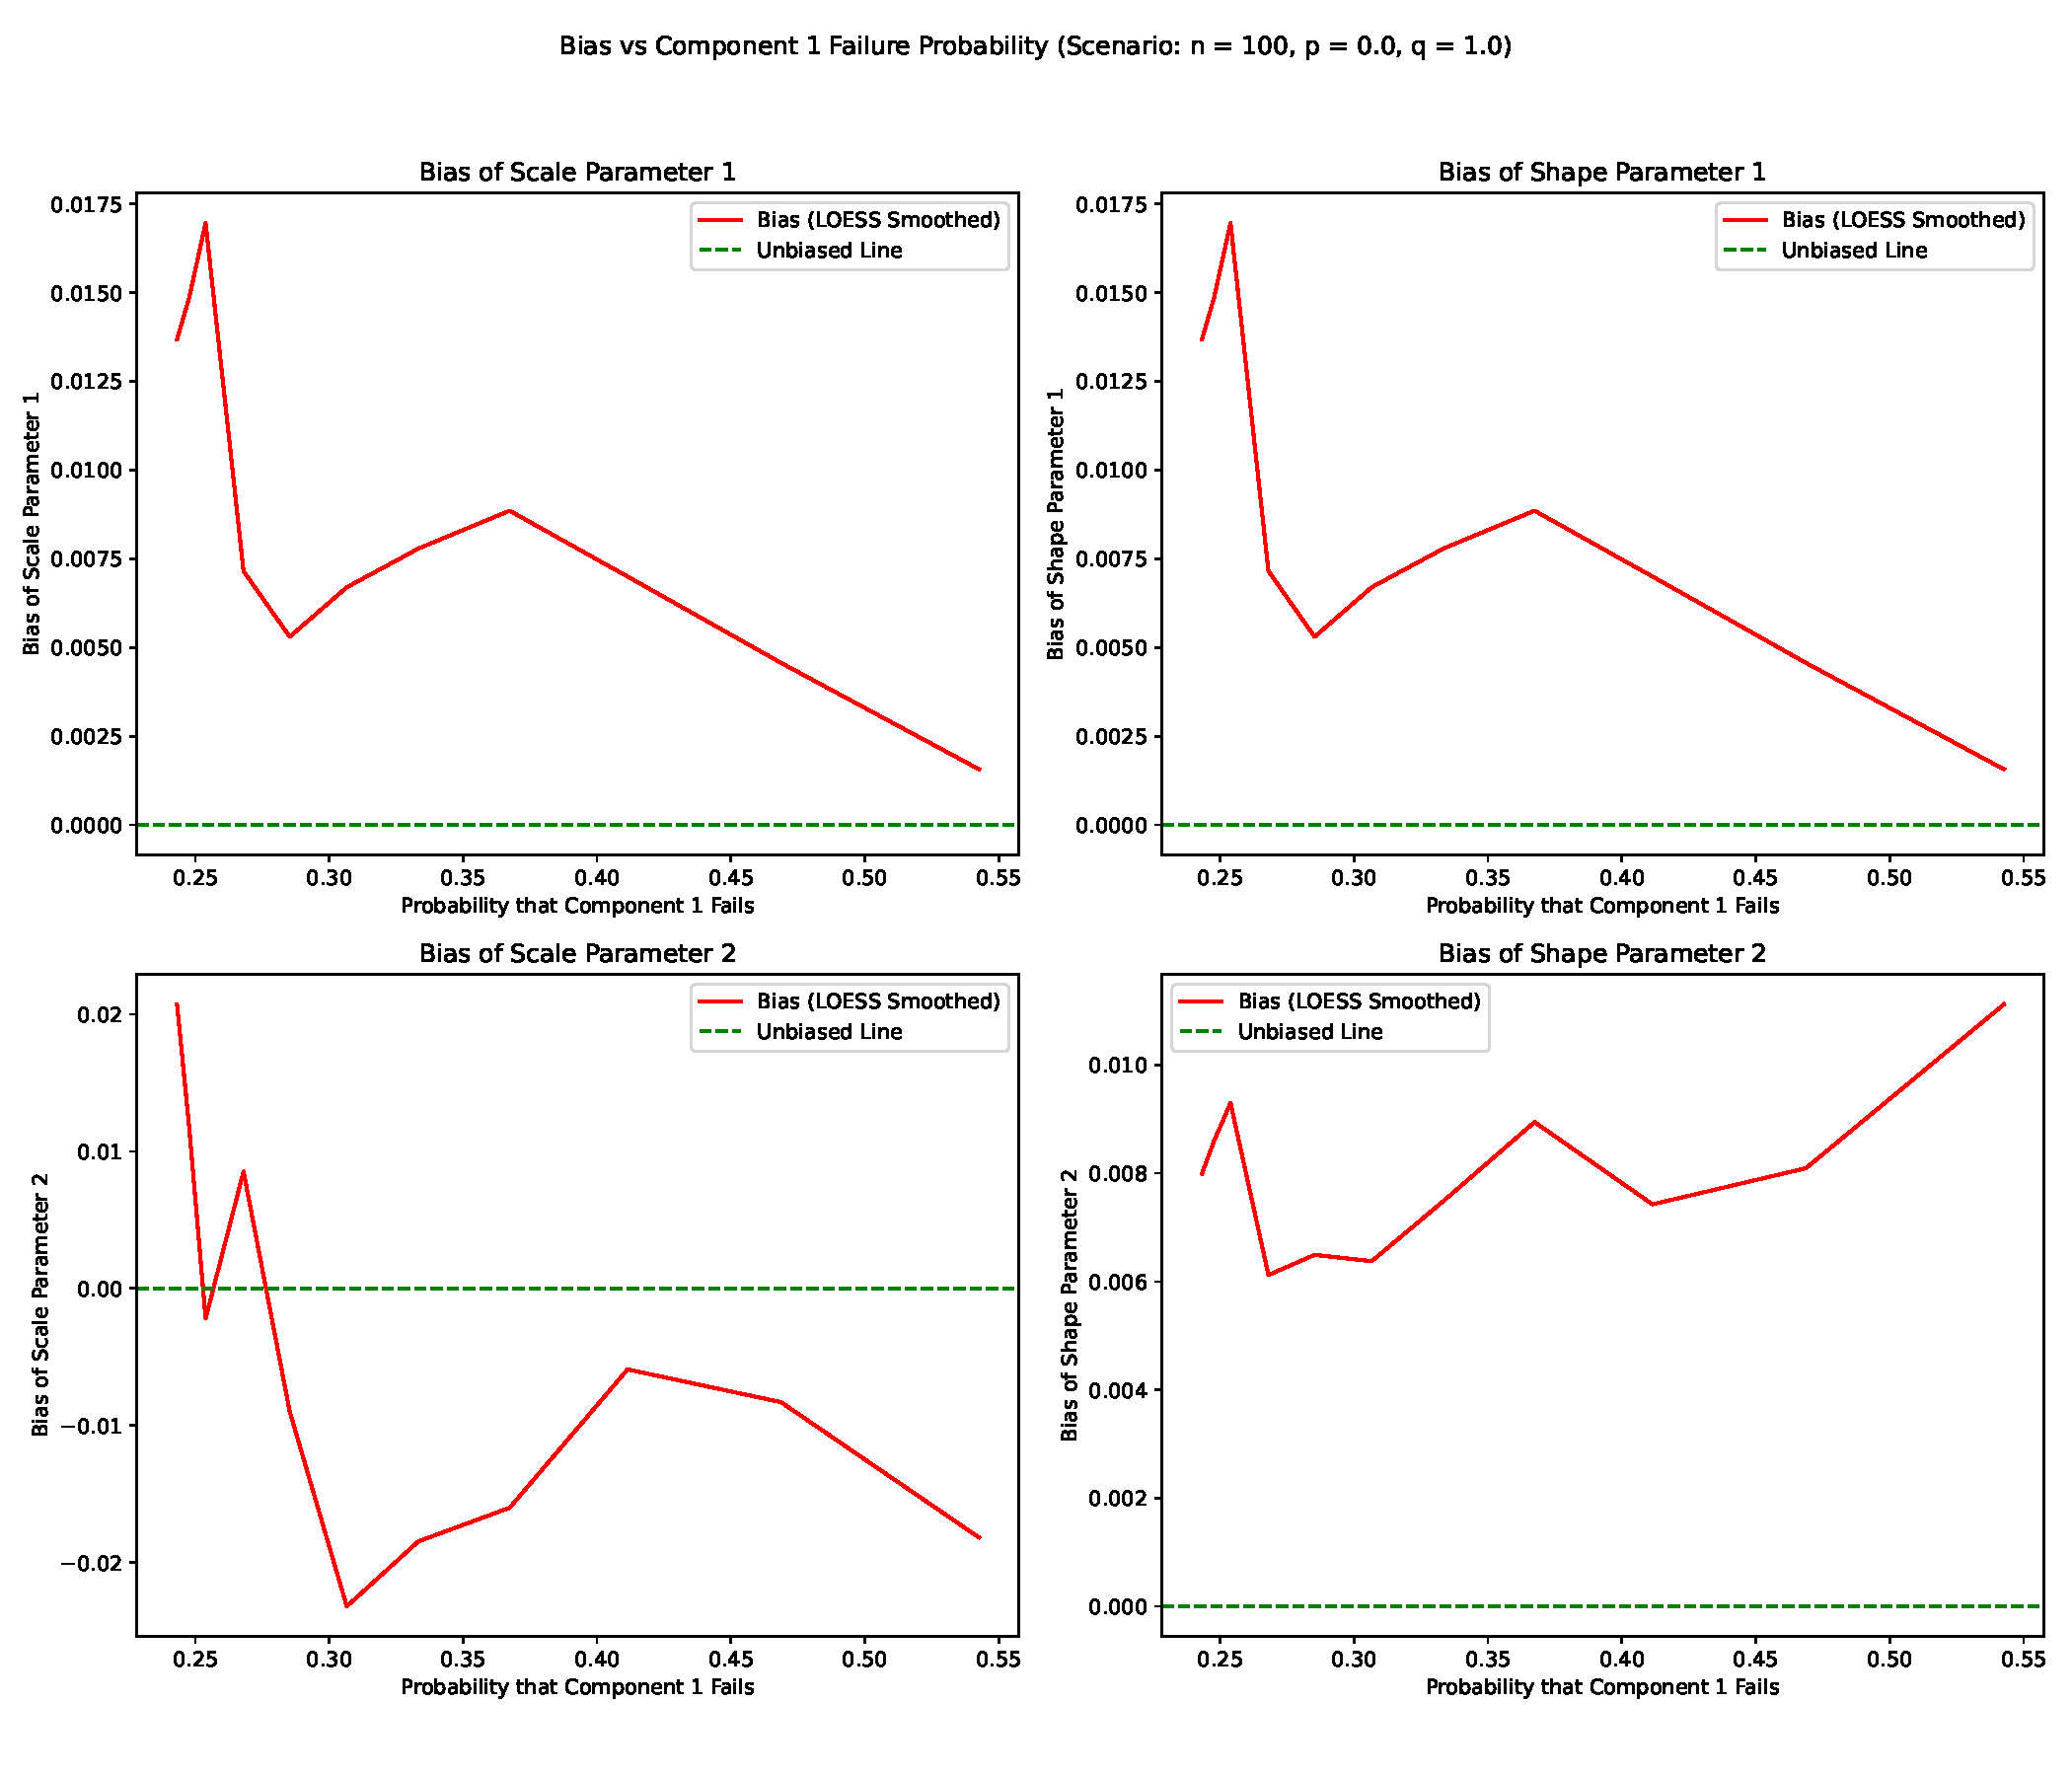
\includegraphics[width=0.85\textwidth]{image/ideal_case_n100_p0_q1.pdf}
\caption{MLE behavior under ideal conditions (no masking, no censoring) for a 2-component series system with $n = 100$.}
\label{fig:ideal-case}
\end{figure}

\section*{Data Availability Statement}

The simulation code and data supporting this study are available in the GitHub repository at \url{https://github.com/queelius/masked-series-model-selection}. The R package used for all simulations is available at \url{https://github.com/queelius/wei.series.md.c1.c2.c3}.

\section*{Conflict of Interest}

The author declares no conflicts of interest.

\bibliographystyle{IEEEtranN}
\bibliography{refs}

\end{document}
